\documentclass{standalone}
\usepackage{tikz}
\usetikzlibrary{patterns, positioning}


\begin{document}
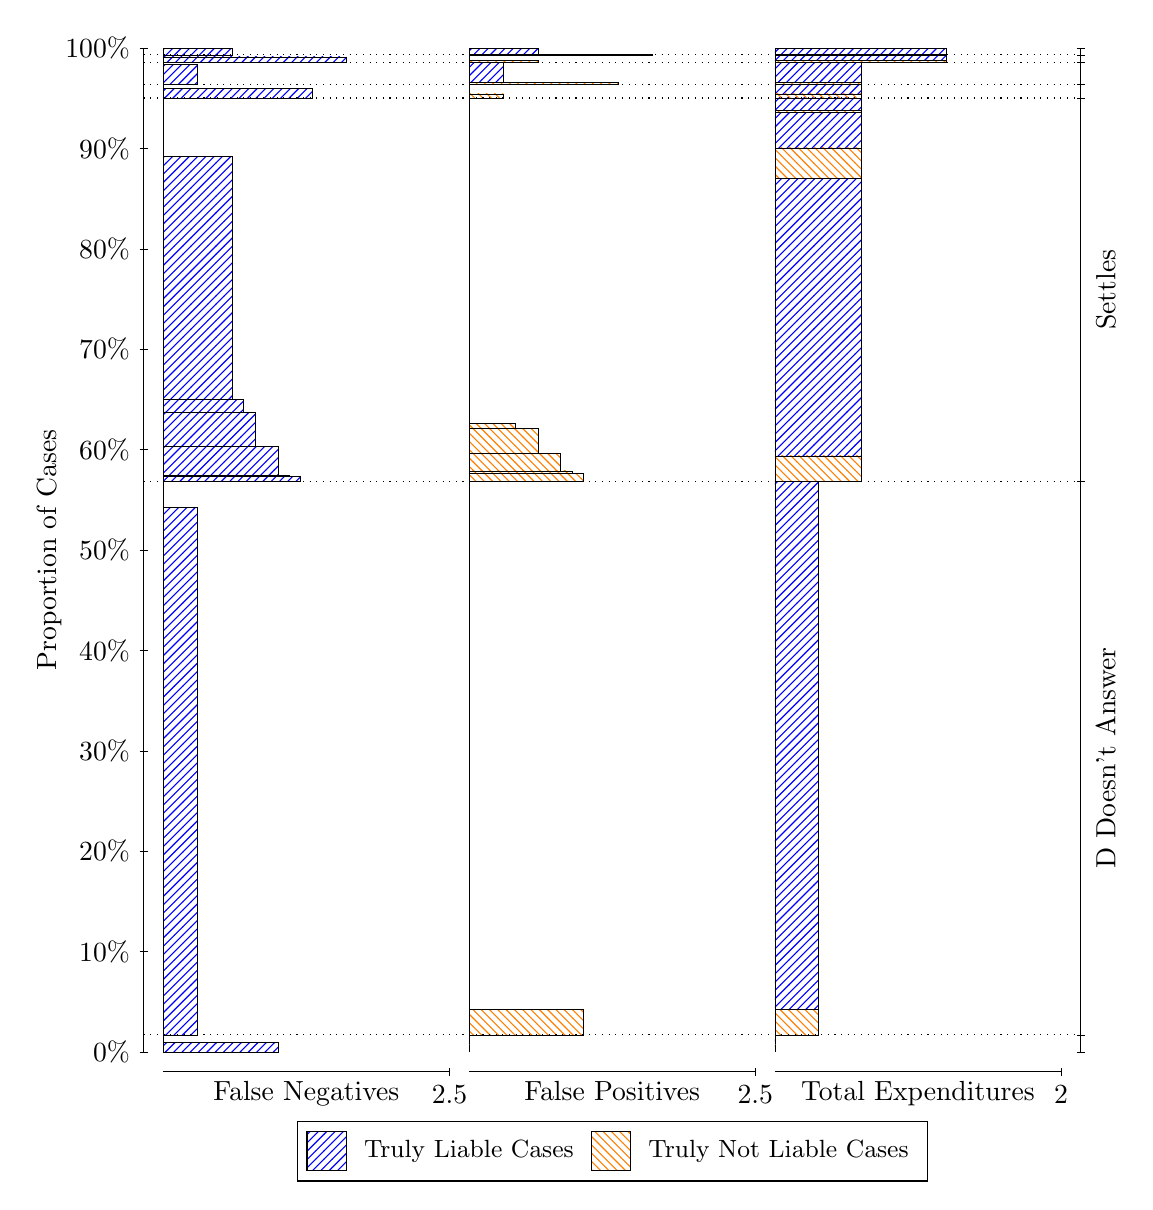
\begin{tikzpicture}
\draw[black, very thin] (1.5,1.75) -- (1.5,14.5);
\node[rotate=90, text=black, anchor=center] at (0.3, 8.125) {Proportion of Cases};
\draw[black, very thin] (1.45,1.75) -- (1.55,1.75);
\node[text=black, anchor=east] at (1.45, 1.75) {0\%};
\draw[black, very thin] (1.45,3.025) -- (1.55,3.025);
\node[text=black, anchor=east] at (1.45, 3.025) {10\%};
\draw[black, very thin] (1.45,4.3) -- (1.55,4.3);
\node[text=black, anchor=east] at (1.45, 4.3) {20\%};
\draw[black, very thin] (1.45,5.575) -- (1.55,5.575);
\node[text=black, anchor=east] at (1.45, 5.575) {30\%};
\draw[black, very thin] (1.45,6.85) -- (1.55,6.85);
\node[text=black, anchor=east] at (1.45, 6.85) {40\%};
\draw[black, very thin] (1.45,8.125) -- (1.55,8.125);
\node[text=black, anchor=east] at (1.45, 8.125) {50\%};
\draw[black, very thin] (1.45,9.4) -- (1.55,9.4);
\node[text=black, anchor=east] at (1.45, 9.4) {60\%};
\draw[black, very thin] (1.45,10.675) -- (1.55,10.675);
\node[text=black, anchor=east] at (1.45, 10.675) {70\%};
\draw[black, very thin] (1.45,11.95) -- (1.55,11.95);
\node[text=black, anchor=east] at (1.45, 11.95) {80\%};
\draw[black, very thin] (1.45,13.225) -- (1.55,13.225);
\node[text=black, anchor=east] at (1.45, 13.225) {90\%};
\draw[black, very thin] (1.45,14.5) -- (1.55,14.5);
\node[text=black, anchor=east] at (1.45, 14.5) {100\%};

\draw[black, very thin] (13.4,1.75) -- (13.4,14.5);
\draw[black, very thin] (13.35,1.75) -- (13.45,1.75);
\node[anchor=west] at (13.35, 1.75) {};
\draw[black, very thin] (13.35,1.9683) -- (13.45,1.9683);
\node[anchor=west] at (13.35, 1.9683) {};
\draw[black, very thin] (13.35,8.9961) -- (13.45,8.9961);
\node[anchor=west] at (13.35, 8.9961) {};
\draw[black, very thin] (13.35,13.866) -- (13.45,13.866);
\node[anchor=west] at (13.35, 13.866) {};
\draw[black, very thin] (13.35,14.034) -- (13.45,14.034);
\node[anchor=west] at (13.35, 14.034) {};
\draw[black, very thin] (13.35,14.32) -- (13.45,14.32);
\node[anchor=west] at (13.35, 14.32) {};
\draw[black, very thin] (13.35,14.413) -- (13.45,14.413);
\node[anchor=west] at (13.35, 14.413) {};
\draw[black, very thin] (13.35,14.5) -- (13.45,14.5);
\node[anchor=west] at (13.35, 14.5) {};

\draw[black, very thin, pattern color=blue, pattern=north east lines] (1.75,1.75) rectangle (3.2033,1.8734);
\draw[black, very thin, pattern color=orange, pattern=north west lines] (1.75,1.8734) rectangle (1.75,1.9683);
\draw[black, very thin, pattern color=blue, pattern=north east lines] (1.75,1.9683) rectangle (2.186,8.6701);
\draw[black, very thin, pattern color=orange, pattern=north west lines] (1.75,8.6701) rectangle (1.75,8.9961);
\draw[black, very thin, pattern color=blue, pattern=north east lines] (1.75,8.9961) rectangle (3.494,9.0648);
\draw[black, very thin, pattern color=blue, pattern=north east lines] (1.75,9.0648) rectangle (3.3487,9.0692);
\draw[black, very thin, pattern color=blue, pattern=north east lines] (1.75,9.0692) rectangle (3.2033,9.4444);
\draw[black, very thin, pattern color=blue, pattern=north east lines] (1.75,9.4444) rectangle (2.9127,9.876);
\draw[black, very thin, pattern color=blue, pattern=north east lines] (1.75,9.876) rectangle (2.7673,10.034);
\draw[black, very thin, pattern color=blue, pattern=north east lines] (1.75,10.034) rectangle (2.622,13.128);
\draw[black, very thin, pattern color=orange, pattern=north west lines] (1.75,13.128) rectangle (1.75,13.866);
\draw[black, very thin, pattern color=blue, pattern=north east lines] (1.75,13.866) rectangle (3.6393,13.983);
\draw[black, very thin, pattern color=orange, pattern=north west lines] (1.75,13.983) rectangle (1.75,14.034);
\draw[black, very thin, pattern color=blue, pattern=north east lines] (1.75,14.034) rectangle (2.186,14.288);
\draw[black, very thin, pattern color=orange, pattern=north west lines] (1.75,14.288) rectangle (1.75,14.32);
\draw[black, very thin, pattern color=blue, pattern=north east lines] (1.75,14.32) rectangle (4.0753,14.388);
\draw[black, very thin, pattern color=orange, pattern=north west lines] (1.75,14.388) rectangle (1.75,14.413);
\draw[black, very thin, pattern color=blue, pattern=north east lines] (1.75,14.413) rectangle (2.622,14.493);
\draw[black, very thin, pattern color=orange, pattern=north west lines] (1.75,14.493) rectangle (1.75,14.5);
\draw[black, very thin, pattern color=orange, pattern=north west lines] (5.6333,1.75) rectangle (5.6333,1.8449);
\draw[black, very thin, pattern color=blue, pattern=north east lines] (5.6333,1.8449) rectangle (5.6333,1.9683);
\draw[black, very thin, pattern color=orange, pattern=north west lines] (5.6333,1.9683) rectangle (7.0867,2.2943);
\draw[black, very thin, pattern color=blue, pattern=north east lines] (5.6333,2.2943) rectangle (5.6333,8.9961);
\draw[black, very thin, pattern color=orange, pattern=north west lines] (5.6333,8.9961) rectangle (7.0867,9.1019);
\draw[black, very thin, pattern color=orange, pattern=north west lines] (5.6333,9.1019) rectangle (6.9413,9.1299);
\draw[black, very thin, pattern color=orange, pattern=north west lines] (5.6333,9.1299) rectangle (6.796,9.3491);
\draw[black, very thin, pattern color=orange, pattern=north west lines] (5.6333,9.3491) rectangle (6.5053,9.6666);
\draw[black, very thin, pattern color=orange, pattern=north west lines] (5.6333,9.6666) rectangle (6.36,9.6695);
\draw[black, very thin, pattern color=orange, pattern=north west lines] (5.6333,9.6695) rectangle (6.2147,9.7337);
\draw[black, very thin, pattern color=blue, pattern=north east lines] (5.6333,9.7337) rectangle (5.6333,13.866);
\draw[black, very thin, pattern color=orange, pattern=north west lines] (5.6333,13.866) rectangle (6.0693,13.917);
\draw[black, very thin, pattern color=blue, pattern=north east lines] (5.6333,13.917) rectangle (5.6333,14.034);
\draw[black, very thin, pattern color=orange, pattern=north west lines] (5.6333,14.034) rectangle (7.5227,14.067);
\draw[black, very thin, pattern color=blue, pattern=north east lines] (5.6333,14.067) rectangle (6.0693,14.32);
\draw[black, very thin, pattern color=orange, pattern=north west lines] (5.6333,14.32) rectangle (6.5053,14.346);
\draw[black, very thin, pattern color=blue, pattern=north east lines] (5.6333,14.346) rectangle (5.6333,14.413);
\draw[black, very thin, pattern color=orange, pattern=north west lines] (5.6333,14.413) rectangle (7.9587,14.42);
\draw[black, very thin, pattern color=blue, pattern=north east lines] (5.6333,14.42) rectangle (6.5053,14.5);
\draw[black, very thin, pattern color=orange, pattern=north west lines] (9.5167,1.75) rectangle (9.5167,1.8449);
\draw[black, very thin, pattern color=blue, pattern=north east lines] (9.5167,1.8449) rectangle (9.5167,1.9683);
\draw[black, very thin, pattern color=orange, pattern=north west lines] (9.5167,1.9683) rectangle (10.062,2.2943);
\draw[black, very thin, pattern color=blue, pattern=north east lines] (9.5167,2.2943) rectangle (10.062,8.9961);
\draw[black, very thin, pattern color=orange, pattern=north west lines] (9.5167,8.9961) rectangle (10.607,9.3211);
\draw[black, very thin, pattern color=blue, pattern=north east lines] (9.5167,9.3211) rectangle (10.607,12.847);
\draw[black, very thin, pattern color=orange, pattern=north west lines] (9.5167,12.847) rectangle (10.607,13.231);
\draw[black, very thin, pattern color=blue, pattern=north east lines] (9.5167,13.231) rectangle (10.607,13.679);
\draw[black, very thin, pattern color=orange, pattern=north west lines] (9.5167,13.679) rectangle (10.607,13.708);
\draw[black, very thin, pattern color=blue, pattern=north east lines] (9.5167,13.708) rectangle (10.607,13.866);
\draw[black, very thin, pattern color=orange, pattern=north west lines] (9.5167,13.866) rectangle (10.607,13.917);
\draw[black, very thin, pattern color=blue, pattern=north east lines] (9.5167,13.917) rectangle (10.607,14.034);
\draw[black, very thin, pattern color=orange, pattern=north west lines] (9.5167,14.034) rectangle (10.607,14.067);
\draw[black, very thin, pattern color=blue, pattern=north east lines] (9.5167,14.067) rectangle (10.607,14.32);
\draw[black, very thin, pattern color=orange, pattern=north west lines] (9.5167,14.32) rectangle (11.697,14.346);
\draw[black, very thin, pattern color=blue, pattern=north east lines] (9.5167,14.346) rectangle (11.697,14.413);
\draw[black, very thin, pattern color=orange, pattern=north west lines] (9.5167,14.413) rectangle (11.697,14.42);
\draw[black, very thin, pattern color=blue, pattern=north east lines] (9.5167,14.42) rectangle (11.697,14.5);
\draw[black, dotted] (1.5,1.9683) -- (13.4,1.9683);
\draw[black, dotted] (1.5,8.9961) -- (13.4,8.9961);
\draw[black, dotted] (1.5,13.866) -- (13.4,13.866);
\draw[black, dotted] (1.5,14.034) -- (13.4,14.034);
\draw[black, dotted] (1.5,14.32) -- (13.4,14.32);
\draw[black, dotted] (1.5,14.413) -- (13.4,14.413);
\draw[black, very thin] (1.75,1.5) -- (5.3833,1.5);
\node[text=black, anchor=north] at (3.5667, 1.5) {False Negatives};
\draw[black, very thin] (5.3833,1.45) -- (5.3833,1.55);
\node[text=black, anchor=north] at (5.3833, 1.45) {2.5};

\draw[black, very thin] (5.6333,1.5) -- (9.2667,1.5);
\node[text=black, anchor=north] at (7.45, 1.5) {False Positives};
\draw[black, very thin] (9.2667,1.45) -- (9.2667,1.55);
\node[text=black, anchor=north] at (9.2667, 1.45) {2.5};

\draw[black, very thin] (9.5167,1.5) -- (13.15,1.5);
\node[text=black, anchor=north] at (11.333, 1.5) {Total Expenditures};
\draw[black, very thin] (13.15,1.45) -- (13.15,1.55);
\node[text=black, anchor=north] at (13.15, 1.45) {2};


\node[text=black, centered, rotate=90] at (13.72, 5.4822) {D Doesn't Answer};
\node[text=black, centered, rotate=90] at (13.72, 11.431) {Settles};





\draw (7.449999999999999,1.5) node[draw=none] (baseCoordinate) {};
\begin{scope}[align=center]
        \matrix[scale=0.5, draw=black, below=0.5cm of baseCoordinate, nodes={draw}, column sep=0.1cm]{
            \node[rectangle, draw, minimum width=0.5cm, minimum height=0.5cm, pattern color=blue, pattern=north east lines] {}; &
            \node[draw=none, font=\small, text=black] (B) {Truly Liable Cases}; &
            \node[rectangle, draw, minimum width=0.5cm, minimum height=0.5cm, pattern color=orange, pattern=north west lines] {}; &
            \node[draw=none, font=\small, text=black] (B) {Truly Not Liable Cases}; \\
            };
\end{scope}

\end{tikzpicture}
\end{document}